 \documentclass{mcmthesis}
 \usepackage{graphicx} % Add this in the preamble
 \usepackage{float}
 \usepackage{longtable}
 \usepackage{lastpage}

\mcmsetup{tstyle=\color{red}\bfseries,
        tcn = 2527095, problem = C, 
        sheet = true, titleinsheet = true, 
        titlepage = false, abstract = true}

  \usepackage{newtxtext,newtxmath}

\usepackage{indentfirst}  
\usepackage{lipsum}

\author{\small \href{https://www.latexstudio.net/}
  {
\includegraphics[width=7cm]{mcmthesis-logo}}}
\date{\today}

\begin{document}
\begin{title}
{Designing Predictive Models for the 2028 Olympics}
\end{title}


\begin{abstract}
\par
The Olympic games are arguably the world's most prominent sports competition of all time, as hundreds of countries from across the globe compete in a series of sports events to demonstrate their national glory and pride. The international significance of these games makes the results all the more momentous. As a result, the practice of forecasting Olympic outcomes in advance has gained significant traction. \par
In our own predictive analysis, we formulate a series of models to predict the characteristics of the upcoming 2028 Summer Olympics in Los Angeles. To simplify our modeling process, we make several simplifying assumptions. We hold notable factors, such as a country's participation, the presence of an event, and an athlete's nationality, constant throughout our analysis. \par
We start with a basic linear regression model. Our model can be considered an adaptation of the naive forecast model in that it only accounts for the total quantity of medals won by a country in its previous Olympic campaign. To run our model, we utilize a dataset containing complete country medal count tables for all previously held summer Olympics from 1896 to 2024. The statistics we obtain for our initial regression line are less than satisfactory, with a mean-squared error of 182.246 and a coefficient of determination ($r^2$) of 0.608. \par
We deduce that a main flaw in our analysis is that our data is excessively longitudinal. It is very likely that the circumstances under which the Olympic games were played in the 1800s have drastically changed compared to today. Therefore, we truncate the years in our dataset starting with the 1864 Olympic games up until 1964. Running the regression model on the new dataset gives us an improved MSE of 81.115 and $r^2$ of 0.820. \par
We transition into our second, improved model where we account for two significant factors. The first factor is the real value of each medal type (based on tier), which we incorporate by running a weighted scoring algorithm on the aforementioned dataset. The second factor is the effect of sport types on individual athlete performance. We implement two additional datasets for this purpose; one contains individual athlete performance across their Olympic campaigns while the other contains categorized counts of Olympic events by sport and discipline. Our new model shows improvement in the MSE (73.087) and $r^2$ (0.839), so we take it as our final model in this paper. \par
Using our improved model, we conduct a variety of analyses for the 2028 summer Olympics, including forecasting a medal table with prediction intervals (RMSE: 8.5491) for the medal count, identifying which countries will earn their first Olympic medals, and discerning trends across countries that emulate the 'great coach' effect. \par


\begin{center}
\end{center}
\end{abstract}



\maketitle
\tableofcontents

\section{Introduction}
\subsection{Background}
In the Olympic Games, thousands of athletes compete not only for individual fame, but also to glorify their country. \par
Predictions for the results of these games is of high importance for many governmental and non-governmental stakeholders. Governments can use the forecasts to identify a nation's athletic success, while businesses and can use these projections to maximize profit. 
[6] \par
Traditionally, Olympic predictions are made closer to the start of the events, relying heavily on the current performance status of athletes [1]. However, researchers across various fields have also introduced a plethora of models to try to predict the results mathematically, including time series and machine learning frameworks [2, 3].

\subsection{Our Work}
We propose two different models that will enable us to characterize the results of the 2028 Summer Olympics in Los Angeles. The second model will be a refined version of the first. \par Before explaining how we derive each model, we elucidate our simplifying assumptions. We then analyze and compare their results collectively, while also noting their individual strengths and potential weaknesses. Finally, we offer suggestions for future work and make several concluding remarks. \par
Through this process, our objective is to achieve the following goals:
\begin{itemize}
    \item Predict the medal table for the 2028 Summer Olympics (number of gold medals and number of total medals) 
    \item Identify which countries are likely to earn their first medal in the upcoming Olympics
    \item Pinpoint a correlation between the events at a given Olympics and the number of medals won by a particular country
    \item Identify the significance of the 'great coach' effect: coaches who transition from one team to another may greatly impact medal counts in individual countries. 
    \item Use our results to inform country Olympic committees
\end{itemize} 

\newpage

\section{Simplifying Assumptions}
To make it easier to analyze our data and create our models, we make the following general assumptions:
\begin{itemize}
    \item Every country that has participated in previous Olympic games will be participating in the 2028 Los Angeles Olympics
    \item Every event that has occurred in previously held Olympic games will be occurring in the 2028 Los Angeles Olympics
    \item Every athlete that has participated in the Olympic games will be participating in the 2028 Los Angeles Olympics, and no athlete will be competing for a different country. However, coaches may compete for a different country.
\end{itemize}

\section{Basic Model}
We begin by presenting a basic model that predicts the medal tables for each participating country in the Olympics. In this model, we isolated the number of Olympic medals won by a country in previous years as the main determining factor.

\subsection{Methodology for the Basic Model}
The standard model used to forecast future Olympic winners is the naive forecast model, which correlates a nation's expected number of medals with their medal count from Olympic games [7]. We take inspiration from this approach by implementing a linear regression model that takes this correlation into account. The rationale behind this strategy was amplified by the fact that we were given historical data of complete country medal count tables for all summer Olympics events from 1896 to 2024. \par
To simplify our model and facilitate our data analysis, we choose to assign equal weights to the medals earned regardless of their tier. In other words, we only considered the total medal count of each country in our basic model. In our improved models, we account for the medal types. Our basic regression model looks like this:
\begin{equation}
y_i(total\ medals) = \beta_o \ + \beta_1 (unweighted\ medals\ last\ olympics_i)
\end{equation} 

\begin{itemize}
    \item $y_i$: Total medals won by country $i$ (what is being predicted).
    \item $\beta_0$: The intercept of the regression model
    \item $\beta_1$: The coefficient representing the impact of medals won in the previous Olympics
    \item Unweighted Medals Last Olympics: Number of medals won by country $i$ in the previous Olympics
\end{itemize}

\subsection{Data Processing for the Basic Model}
To run our linear regression model, we need to clean our data and reproduce it in a format that would allow for extensive testing. We manipulate the historical data of complete country medal count tables in Python by appending an extra column to the dataset named 'medals\textunderscore won\textunderscore previous\textunderscore year'. This column recursively updates the number of medals won by a country in their most recent Olympics based on the current year that we are parsing through. In addition, we truncate the 'Rank', 'Gold', 'Silver', and 'Bronze' columns of the dataset, as they are not needed in our basic model. 

\subsection{Results from the Basic Model}
In Figure 1 we display a regression graph obtained by accounting for all previously played Olympic games. In the figure, the y-values of each blue dot represent predictions for a country's projected medal count in the upcoming Olympic games, depending on their results in the last Olympics. The red line represents our regression line, which we generated using the Sci-Kit library in Python. \par
\begin{figure}[h] % 'h' stands for 'here'; other options include 't', 'b', 'p'
    \centering
    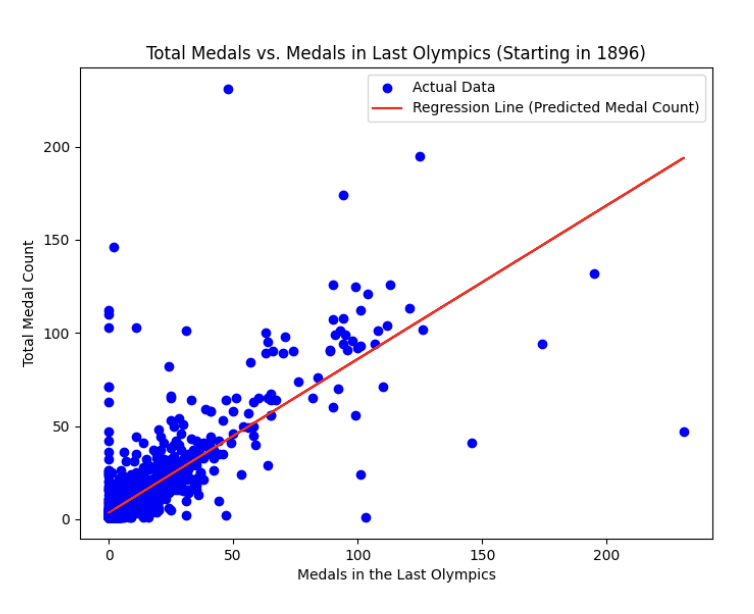
\includegraphics[width=0.6\textwidth]{figures/Regression_Grpah_Two.png}
    \caption{The regression graph depicting the predicted number of Olympic medals won by each country based on their results in the preceding Olympic games. The data spans from the emergence of the games in 1896 to the most recent games played in 2024.}
    \label{fig:image2}
\end{figure}
To assess the fit of this regression model, we calculate the mean-squared error (MSE) and the coefficient of determination ($r^2$). A lower MSE indicates that the model's medal predictions are closer to the actual medal predictions, while a higher $r^2$ indicates that the model explains a larger proportion of the variability in the predicted number of medals. \par
We obtain 182.246 for our MSE and 0.608 for our $r^2$. While these are respectable values, we hypothesize that the defects in these values may be due to unobservable factors, including but not limited to:
\begin{itemize}
    \item Changes in the events held at the Olympics over time
    \item Changes in the athletes participating in the Olympics over time
    \item Participation variance across individual countries over time
\end{itemize} \par
To somewhat counteract this imperfection, we truncate a portion of the earlier years in the dataset. Table 1 displays the $r^2$ values obtained from incrementally truncating the results from previous competitions. We begin with the 1896 Olympic games as we perceive its results to be the least representative of our predictions. \par

\begin{table}[h!]
\centering
\begin{tabular}{|c|c|}
\hline
\textbf{Year} & \textbf{\( r^2 \) Value} \\ \hline
1900          & 0.613                    \\ \hline
1916          & 0.746                    \\ \hline
1932          & 0.748                    \\ \hline
1948          & 0.777                    \\ \hline
1964          & 0.819                    \\ \hline
1972          & 0.814                    \\ \hline
1980          & 0.802                    \\ \hline
\end{tabular}
\caption{Yearly \( r^2 \) Values}
\label{tab:r2_values}
\end{table}


We ascertain from Table 1 that our model peaked after truncating all results prior to 1964, as we obtain our highest $r^2$ value of 0.820. Indeed, as Figure 2 shows, our data is better represented upon this change with a lower MSE of 81.115 and a higher $r^2$ of 0.820. \par
\begin{figure}[h] % 'h' stands for 'here'; other options include 't', 'b', 'p'
    \centering
    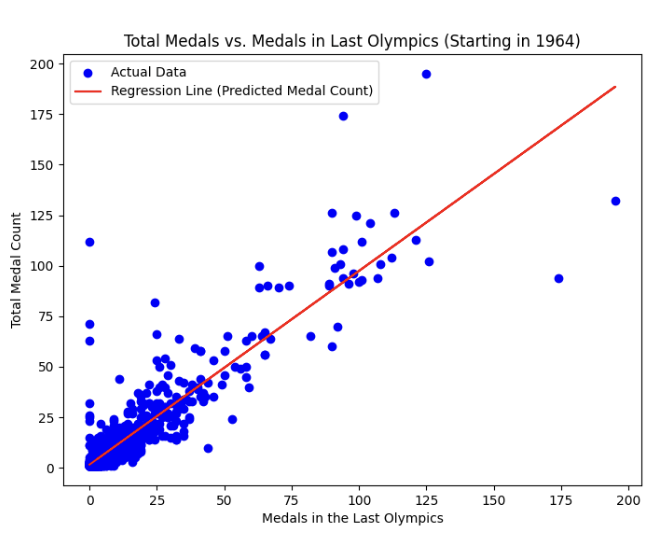
\includegraphics[width=0.6\textwidth]{figures/Regression_Graph_One.png}
    \caption{The regression graph depicting the predicted number of Olympic medals won by each country based on their results in the preceding Olympic games. The data spans from the emergence of the games in 1964 to the most recent games played in 2024.}
    \label{fig:image2}
\end{figure}
\subsection{Limitations of the Basic Model}
The simple linear regression model we have introduced is a good starting point for our tasks. However, the model does not incorporate several factors we perceive to be significant in characterizing the results of future Olympic games, including:
\begin{itemize}
    \item The value of each type of medal won
    \item The variance in individual athlete capabilities
    \item The unique effect of hosting the games for a specific country
\end{itemize} \par
Another main issue with our simple model is that it does not satisfactorily represent the countries that have yet to earn a medal. In fact, Figure 2 shows that the model is skewed by the countries that have won the most medals. In our upcoming models, we integrate the aforementioned factors in our predictions and address this issue. 
\newpage
\section{Improved Model}
In the basic model, we only utilized the total number of medals won by a country in the previous Olympic games to predict their medal count in the next Olympic games. We now factor in two more aspects into our model to improve its validity:
\begin{itemize}
    \item The value of each medal type (gold, silver, bronze)
    \item Individual athlete performance (based on event characteristics and their previous results in these events)
\end{itemize}
\subsection{Methodology for the Improved Model}
Typically, higher levels of achievement are directly correlated with a higher chance of future success. Many national governments will typically value medals of higher tiers than those of lower tiers, which can impact their future investment towards success in the succeeding Olympics. This motivates us to assign greater weights to the medals belonging to higher tiers (e.g. gold) in our linear regression model. \par 
In addition, many athletes participate in the Olympic games multiple times, and some even participate in multiple events at a time. An athlete who has achieved more in previous games than an inferior or inexperienced athlete may bolster a country's chances of winning more medals. Furthermore, the specific events that these athletes partake in may be more popular than others. We attempt to quantify how the popularity of specific Olympic events affects the performance of athletes, which in turn affects their nation's medal count. \par
To reinforce our model, we will only be analyzing the data for the Olympic games played from 1964 to 2024. Based on our analysis of the basic model, we assume that implementing data prior to 1964 will undermine our future models as well. 

\subsection{Data Processing for the Improved Model}
To refine our linear regression model, we account for medal type and individual athletes. We are given two valuable datasets (Dataset A, Dataset B) that we use to facilitate our model. Dataset A lists the sport, year of participation, and results of all athletes that have participated in the Olympics, while Dataset B displays counts of the number of events by sport and discipline for all previous Olympic games. \par
To represent medal types, we develop a scoring system in Python that assigns greater weights to medals of higher accomplishment. Starting with the bronze tier, we choose to recursively assign weights where the value of the next tier is twice the value of the previous tier. This leads us to the following difference equation

\begin{equation}
x_{n+1} = 2\,x_n \quad \text{for} \quad n = 1, 2, 3,\dots
\end{equation}

where $x$ represents the weight we assign to the medal and $n$ represents the tier level. The tier corresponding to $n = 1$ is the bronze tier with an initial value of 0.5. Naturally, a greater $n$ corresponds to a higher tier. We will also manually assign 0 to an athlete who did not earn any medal. With this factor implemented into our model, our regression equation now looks like this: 

\begin{equation}
y_i(total\ medals) = \beta_o \ + \beta_1 (weighted\ medals\ last\ olympics_i)
\end{equation} 

\begin{itemize}
    \item $y_i$: Total medals won by country $i$ (what is being predicted)
    \item $\beta_0$: The intercept of the regression model
    \item $\beta_1$: The coefficient representing the impact of weighted medals won in the previous Olympics
    \item Weighted Medals Last Olympics: The weighted average of the number of gold, silver, and bronze medals won in the previous Olympics for country $i$
\end{itemize}

\par
To account for individual events and athletes, we choose to assign each country with an athlete-weight value. To do this, we first implement a Python program that uses Dataset B to identify the most popular types of sports played in previous Olympic games. Upon cleaning the dataset, we discover that three types held a significantly greater number of events compared to other types of sports:
\begin{enumerate}
    \item Athletics: 684 total events from 1964 - 2024
    \item Aquatics: 627 total events from 1964 - 2024
    \item Gymnastics: 257 total events from 1964 - 2024
\end{enumerate} \par
This finding motivates us to attribute greater values to those athletes that participate in events in these categories. We decide to assign weights of 0.75 to athletes in the 'Athletics' and 'Aquatics' programs, 0.25 to athletes in the 'Gymnastics' program, and 0.1 to athletes not in any of these programs. To do this, we clean the data in Dataset A, extracting information for each athlete as well as the characteristics of their participation throughout the Olympics. We then assign each country a total score, and integrate each country's individual score into our regression model. Table 2 displays a portion (1992 - 2012) of the results obtained from applying this weighting system to all participating athletes from the 1964 games and onward. In mathematical terms, our regression model now looks like this: 


\begin{equation}
y_i(total\ medals) = \beta_o \ + \beta_1 (weighted\ medals\ last\ olympics_i) \ + \beta_2(weighted\ athlete\ value_i)
\end{equation} 

\begin{itemize}
    \item $y_i$\ : Total medals won by country $i$ (what is being predicted).
    \item $\beta_0$: The intercept of the regression model
    \item $\beta_1$: The coefficient representing the impact
    of weighted medals won in the previous Olympics
    \item $\beta_2$: The coefficient representing the impact
    of weighted athlete value for country $i$
    \item Weighted Medals Last Olympics: The weighted average of the number of gold, silver, and bronze medals won in the previous Olympics for country $i$
    \item Weighted Athlete Value: The weighted average of the number of aquatics, athletics, gymnastics, and other athletes for country $i$
\end{itemize}


\begin{table}[H]
\centering
\resizebox{\textwidth}{!}{%
\begin{tabular}{|c|c|c|c|c|c|}
\hline
\textbf{Year} & \textbf{Aquatics Athletes} & \textbf{Athletics Athletes} & \textbf{Gymnastics Athletes} & \textbf{Other Athletes} & \textbf{Weighted Athlete Value} \\ \hline
1992          & 42                                & 38                                & 84                                & 214                           & 351                           \\ \hline
1996          & 48                                & 36                                & 91                                & 243                           & 380.5                         \\ \hline
2000          & 49                                & 32                                & 74                                & 237                           & 354.5                         \\ \hline
2004          & 59                                & 55                                & 72                                & 304                           & 452                           \\ \hline
2008          & 65                                & 69                                & 62                                & 512                           & 586                           \\ \hline
2012          & 77                                & 52                                & 45                                & 289                           & 447.5                         \\ \hline
\end{tabular}%
}
\caption{Breakdown of number of different event athletes and weighted athlete values for China from 1992 - 2012}
\label{tab:china_athletes}
\end{table}


\subsection{Results from the Improved Model}
Before presenting the improved model, we find it useful to analyze the individual effects of both factors. In Figures 3 and 4 we display the regression graphs obtained from accounting for our new factors in separate models. In both figures, the y-values of each blue dot denote predictions for country's medal count in the upcoming Olympic games. As in the previous figures, the red lines represent our regression lines, which we generated using Sci-Kit. 
\begin{figure}
     \centering
     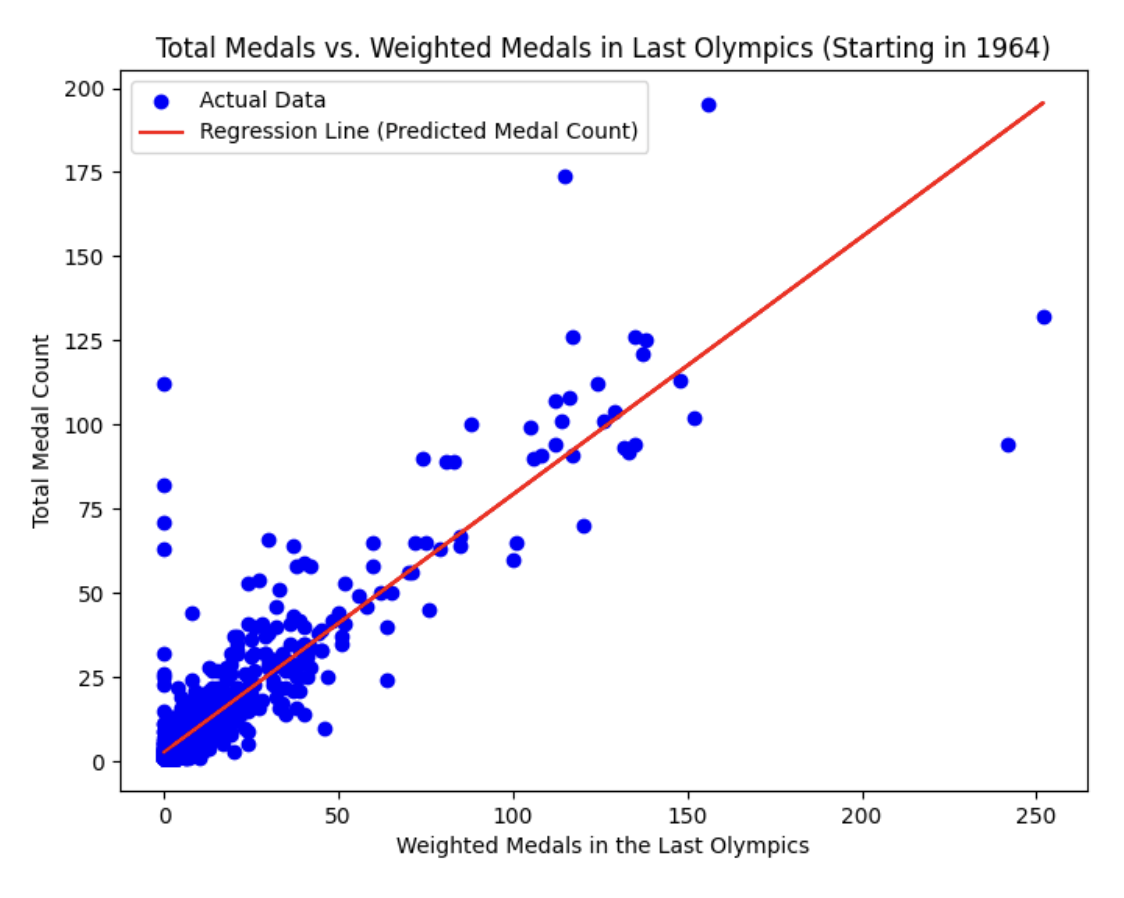
\includegraphics[width=\textwidth]{figures/Regression_Graph_Three.png}
     \caption{The regression graph depicting the predicted number of Olympic medals won by each country based on their results in the preceding Olympic games, taking into account the weights of the medals themselves. The data spans from the emergence of the games in 1964 to the most recent games played in 2024.}
     \label{fig:image 3}
\end{figure}
\begin{figure}
     \centering
     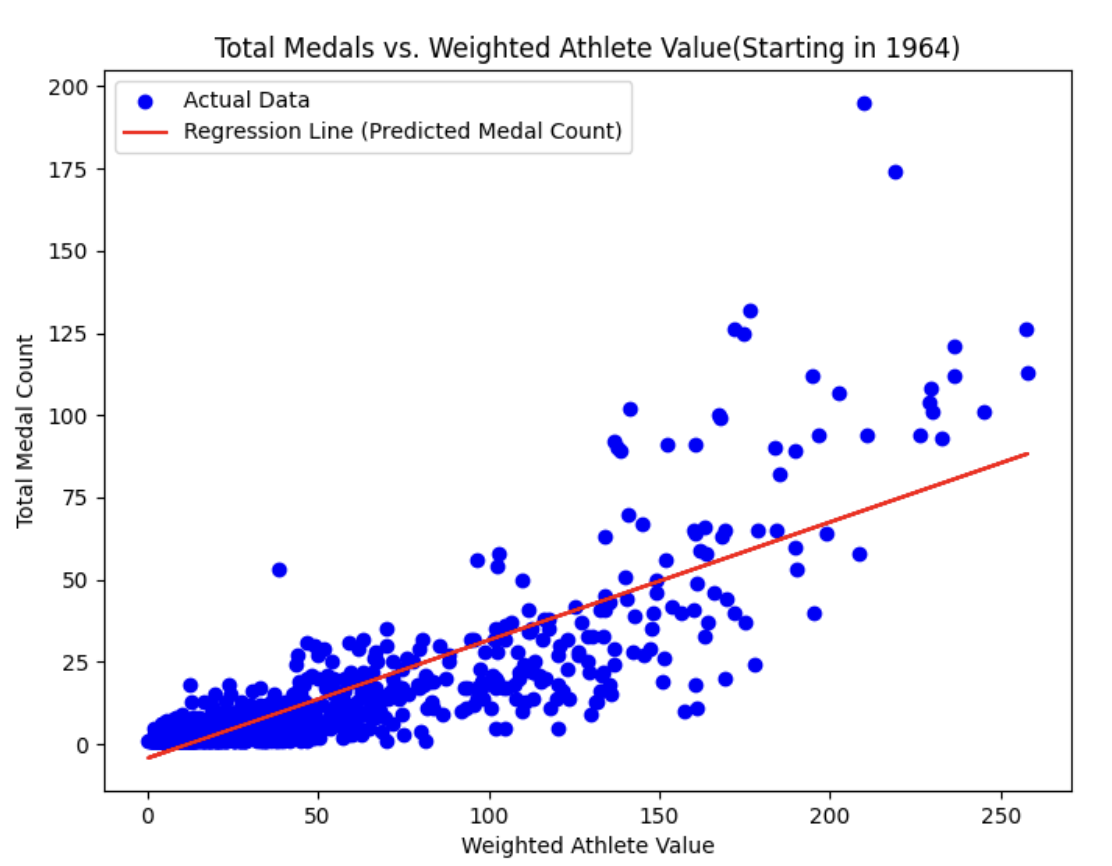
\includegraphics[width=\textwidth]{figures/Regression_Graph_Four.png}
     \caption{The regression graph depicting the predicted number of Olympic medals won by each country based on total weighted athlete values, taking into account the popularity of the events each individual athlete partakes in. The data spans from the emergence of the games in 1964 to the most recent games played in 2024.}
     \label{fig: image 4}
\end{figure} \par
As with the basic model, we use the MSE and the value of $r^2$ to qualify the fit of our regression models. For our regression model that accounts for weighted medals, we obtain a MSE of 89.688 and an $r^2$ of 0.801. Similarly, we obtain a MSE of 138.959 and an $r^2$ of 0.694 for our model that implements weighted athlete values. Interestingly, both regression graphs seem to fit the data worse. We hypothesize that this may simply be because we did not consider both factors collectively. \par
We now give the results obtained from accounting for both figures simultaneously in our regression model (4). Since we have introduced multiple independent variables in our regression model, a regression graph would not be easy to visually interpret. Therefore, we omit the graph from our paper. \par
Our improved regression model yields an improved MSE of 73.087 and an improved $r^2$ of 0.839. Both values are comparably better to those obtained from our basic model, indicating that our positive model is a stronger predictor of future Olympic results. 

\subsection{Limitations of the Improved Model}
Despite the inherent improvements in our improved regression model, we acknowledge several limitations on it that undermine its validity. We offer several possibilities on how to resolve them. \par 
Firstly, the model assumes that each athlete competing in the Olympics remains in constant condition throughout each edition of the games that they partake in. Realistically, the conditions of athletes change over time due to a variety of unobservable factors such as age and injury. This should have a noticeable impact on their performance, which could potentially alter our weighted athlete values. To obtain a better sense of how the changing conditions of athletes will modify our results, we would need to introduce a new variable that models the alterations in an athlete's performance over time. \par
Another weakness of our model is that it assumes that all medals of a particular type hold equal weight. As we noted, some Olympic events are held more frequently than others due to their heightened popularity or preference by a host country. This would appreciate the value of gold medals earned in these events relative to those earned in lesser-regarded events. However, we disregard this factor in our model. To account for its effects, we could implement an algorithm that assigns weights to medals based on both their type and how well regarded they are by a country. \par

\section{Model Insights and Analysis}
\subsection{Predicted Medal Table for the 2028 Los Angeles Olympics}
Using our improved regression model (4), we give our best prediction for the medal table for the upcoming Olympic games. In table 3 we display our results. Not only do we enumerate the predicted total number of medal for each country, but we also list our prediction intervals next to the total. \par
As table 3 shows, many countries that have previously achieved success at the games are projected to achieve similar levels of success in the upcoming Olympic games. However, as we noted before, we feel that our model does not fully represent those countries with minimal prior success. We attempt to address this concern in a future section. 
\newpage

\begin{longtable}{rccc}
\toprule
 & Name & Predicted Total Number Medals & Predicted Medal Range \\
\midrule
1 & United States & 110 & [102, 119] \\
2 & China & 83 & [74, 91] \\
3 & Great Britain & 63 & [55, 72] \\
4 & Japan & 59 & [51, 68] \\
5 & Australia & 57 & [49, 66] \\
6 & France & 51 & [43, 60] \\
7 & Italy & 48 & [40, 57] \\
8 & Germany & 46 & [38, 55] \\
9 & Canada & 37 & [28, 45] \\
10 & Netherlands & 37 & [29, 46] \\
11 & Spain & 28 & [19, 36] \\
12 & Brazil & 28 & [19, 37] \\
13 & Poland & 25 & [16, 33] \\
14 & Hungary & 21 & [12, 29] \\
15 & New Zealand & 18 & [10, 27] \\
16 & Switzerland & 16 & [8, 25] \\
17 & Belgium & 14 & [6, 23] \\
18 & Jamaica & 14 & [6, 23] \\
19 & Sweden & 14 & [5, 22] \\
20 & Ukraine & 13 & [4, 21] \\
21 & Kenya & 12 & [3, 20] \\
22 & Ireland & 11 & [2, 19] \\
23 & Cuba & 11 & [3, 20] \\
24 & Norway & 10 & [1, 18] \\
25 & South Africa & 9 & [0, 18] \\
26 & Denmark & 9 & [1, 18] \\
27 & Israel & 9 & [0, 17] \\
28 & India & 8 & [0, 16] \\
29 & Greece & 8 & [0, 17] \\
30 & Serbia & 7 & [0, 16] \\
31 & Chinese Taipei & 6 & [0, 14] \\
32 & Slovenia & 6 & [0, 14] \\
33 & Croatia & 6 & [0, 15] \\
34 & Austria & 5 & [0, 13] \\
35 & Uzbekistan & 5 & [0, 13] \\
36 & Mexico & 5 & [0, 13] \\
37 & Bulgaria & 5 & [0, 13] \\
38 & Portugal & 5 & [0, 14] \\
39 & Ethiopia & 5 & [0, 13] \\
40 & Egypt & 5 & [0, 14] \\
41 & Romania & 5 & [0, 14] \\
42 & Uganda & 4 & [0, 13] \\
43 & Ecuador & 4 & [0, 13] \\
44 & Colombia & 4 & [0, 13] \\
45 & Kazakhstan & 4 & [0, 12] \\
46 & Georgia & 4 & [0, 12] \\
47 & Argentina & 3 & [0, 12] \\
48 & Dominican Republic & 3 & [0, 11] \\
49 & Lithuania & 3 & [0, 11] \\
50 & Azerbaijan & 2 & [0, 10] \\
51 & Slovakia & 2 & [0, 11] \\
52 & Philippines & 2 & [0, 10] \\
53 & Morocco & 2 & [0, 11] \\
54 & Singapore & 1 & [0, 10] \\
55 & Botswana & 1 & [0, 9] \\
56 & Chile & 1 & [0, 10] \\
57 & Algeria & 1 & [0, 10] \\
58 & Kosovo & 1 & [0, 9] \\
59 & Thailand & 1 & [0, 9] \\
60 & Tunisia & 1 & [0, 9] \\
61 & Indonesia & 1 & [0, 10] \\
62 & Qatar & 1 & [0, 10] \\
63 & Puerto Rico & 1 & [0, 10] \\
64 & Mongolia & 1 & [0, 9] \\
65 & Peru & 1 & [0, 10] \\
66 & Albania & 0 & [0, 7] \\
67 & Cabo Verde & 0 & [0, 7] \\
68 & Bahrain & 0 & [0, 9] \\
69 & Armenia & 0 & [0, 9] \\
70 & Guatemala & 0 & [0, 8] \\
71 & Dominica & 0 & [0, 7] \\
72 & Cyprus & 0 & [0, 8] \\
73 & Fiji & 0 & [0, 9] \\
74 & Grenada & 0 & [0, 8] \\
75 & Malaysia & 0 & [0, 8] \\
76 & Kyrgyzstan & 0 & [0, 9] \\
77 & Jordan & 0 & [0, 8] \\
78 & Pakistan & 0 & [0, 7] \\
79 & Saint Lucia & 0 & [0, 7] \\
80 & Panama & 0 & [0, 8] \\
81 & Tajikistan & 0 & [0, 8] \\
82 & Zambia & 0 & [0, 9] \\
\bottomrule
\caption{Our predicted medal table for the 2028 Summer Olympics based on (4)}
\end{longtable}

\subsection{Final Result Analysis}

When comparing the predictions for 2028 to the results from 2024, the top three countries—USA, China, and Great Britain—remain in the same order. However, all three see a decline in their total medal counts, with the USA predicted to win 16 fewer medals compared to 2024. Below the top three, there are notable changes. Japan makes a significant leap from 6th place in 2024 to 4th place in 2028, with a predicted increase of 14 medals. This improvement can likely be attributed to the fact that, while Japan ranked 6th in total medals in 2024, they secured 20 gold medals, placing them 3rd in the gold medal ranking. The improved model's consideration of medal weightage as a factor highlights Japan's improvement.

\par Germany sees a smaller positional jump, moving from 9th to 8th, but their total medal count increases significantly, from 33 to 46—a gain of 13 medals. Spain also experiences upward momentum, moving from 15th to 11th place with a 10-medal increase. Most other countries, particularly those in the lower rankings, see little movement, with many maintaining their 2024 positions. 

\par The medal range intervals in this model were determined by the RMSE (root-mean-squared-error) of the multiple regression model. The value of the RMSE was 8.5491, which shows that our model's predictions, on average, would be off by 8.5491 medals, as shown in the medal intervals.

\textbf{Strengths of the Model} 

\par This model excels in its ability to better represent mid-table countries (approximately ranked 7th to 27th) by emphasizing medal weightage and the number of athletes in high-value events. This approach provides a more rigorous analysis of how countries perform in events that historically yield higher medal counts. For example, the emphasis on gold, silver, and bronze weightage helped explain Japan's improvement in the rankings, even with fewer total medals than other countries in 2024. 

Additionally, by focusing on athlete counts in specific events with higher medal weightage, the model offers deeper insights into how these factors influence a country's overall medal tally. This detailed analysis provides a more nuanced understanding of mid-tier countries' performances, helping to predict meaningful jumps (or declines) in rankings based on the types of medals won, rather than total counts alone. 

\textbf{Weaknesses of the Model}

This model struggles to account for countries with very few or no prior medals. While the inclusion of an athlete-weight factor was intended to address this gap, it did not significantly improve predictions for lower-ranked countries. This limitation leaves some smaller nations underrepresented in the analysis. 

Additionally, the model places a heavy emphasis on the top three medal-winning events, which may not fully capture the performances of countries excelling in other events. For instance, some countries have strong individual athletes who perform consistently in niche events that do not yield a large number of medals overall but are still important. By overlooking such scenarios, the model may miss subtle but valuable contributions from these athletes. A more detailed model could address these nuances and enhance its accuracy.


\subsection{Countries To Earn Their First Medal at the Next Olympics}
A unique procedure we can perform on our datasets is to analyze countries who currently have no medals of any type and to find the first three to most likely earn a medal in the 2028 Los Angeles Olympics. We use dataset A to do this by combing through and sorting this data through the Excel Power Query Editor. Athletes that represent respective countries with any type of medal ("Gold", "Silver", "Bronze") were automatically removed, giving us a modified dataset of countries with zero medals which we denote ($\gamma$). Using ($\gamma$), we then quantify the number of athletes representing each country, as well as their respective events using the command: 

\par
\textit{if [Team] = "(respective zero medal team)" return 1,
        else return 0} \par

The 1 and 0 category was then refined and sorted using the "Group By" function, resulting in a more filtered dataset of zero-medal countries. A benchmark was also used to eliminate countries with relatively lower athletes, by grouping the country and athlete count again and marking the data cell if the count exceeded a 90 percentile range. The marked data cells composed a new set of countries with high athlete counts that was compared extensively.
\par
The event "Football" was eliminated due to the reasoning that such an event required a high quantity of athletes that was weakly correlated to potential performance. With this in mind, a trend line of the number of athletes each country had in each year was compared and we found that \textbf {Angola, Guinea, and Iraq} showed the most significant growth and relevance in Olympic participation. According to our model, these three countries are most likely to earn their first medal in the upcoming Olympics.  
\subsection{Event Popularity} 
We wish to clarify the rationale behind factoring in the popularity of individual events into our improved model. As explained earlier, we tried to incorporate athlete performance into our revised model by accounting for the relative popularity of their corresponding events. However, one factor that we wish to incorporate in future models is the biased effect towards host nations in the Olympic games. A host nation may play a stronger role in deciding which games are played; if they prefer hosting certain events over others, this could skew the results of the games in their favor. Although we were unable to include the host nation as a factor in our model, we believe that this is relatively easy to implement; we would just assign an extra weighted value towards the host nation for each edition of the Olympic games. 

\subsection{Great Coach Effect} 

A well received phenomenon in sports culture is the impact of a 'great coach' effect on a team's performance. It is believed that the mere presence of a coach with previous merits or a strong reputation can uplift a struggling team to glory. While some associate this team's sudden success with the heightened excellence of the coach, others refer to psychological effects that renowned coaches bring to their teams [8]. We attempt to pinpoint trends in our data that resemble this 'great coach' effect. Through extensive testing on Dataset A, we extract three countries with minimal prior medal success that could significantly benefit from the impact of a 'great coach' in specific sports.

\textbf{Country 1: India in Athletics}

In 2024, India had 32 athletes competing in athletics events, as indicated by the cleaned dataset with weighted athlete values. However, only one of these athletes, Neeraj Chopra, secured a medal (Silver in Javelin Throw). Improving the coaching staff could significantly enhance India's athlete-to-medal ratio in athletics.

India's 2024 Athlete-to-Medal ratio: $1/32$ or $0.0313$

Assumptions: We assume that India sends all 32 athletes to the athletics events in 2028. As illustrated in table 4, having a great coach could double or triple India's current athlete-to-medal ratio. 

\begin{equation}
    Medal\ Count \ = Total\ Athletes\ \times \ Athlete \textnormal- to \textnormal- Medal\ ratio
\end{equation}

\begin{center}
Medal Distribution (based on assumption): \\
Gold = 20\% chance \\
Silver = 30\% chance \\
Bronze = 50\% chance
\end{center}

\begin{table}[H]
\centering
\begin{tabular}{|c|c|c|}
\hline
\textbf{Athlete-to-Medal Ratio} & \textbf{Total Medals Won} & \textbf{Gold, Silver, Bronze} \\ \hline
0.0313 (2024 Real) & 1 & 0, 1, 0 \\ \hline
0.0626 (Doubled projection)   & 2 & 0, 1, 1 \\ \hline
0.0939 (Tripled projection)   & 3 & 1, 1, 1 \\ \hline
\end{tabular}
\caption{Athlete-to-Medal ratio and corresponding medal counts for India in athletics with improved coaching.}
\label{tab:athlete_medal_ratio}
\end{table}
In the best case scenario, India could win approximately 1 gold, 1 silver, and 1 bronze medal in 2028 with better coaching. 

\textbf{Country 2: Brazil in Swimming}

In 2024, Brazil had 39 athletes competing in swimming events but failed to win any medals. This remarkably low athlete-to-medal ratio could potentially be improved with enhanced coaching.

Brazil's 2024 athlete-to-medal ratio: 0/39 or 0.00

Assumptions: We assume that Brazil sends all 39 athletes to swimming events in 2028, and that there could be a 10\% increase in performance with better coaching. 

With a 10\% increase:

Medal Count = $39\ \times\ 0.1 = 3.9$ medals 

\begin{itemize}
\item Gold Medals = $3.9\ \times\  0.2 = 0.78$ 
\item Silver Medals = $3.9\ \times\  0.3 = 1.17$ 
\item Bronze Medals  = $3.9\ \times\  0.5 = 1.95$ 
\end{itemize}

In 2028, Brazil could win approximately 1 gold, 1 silver, and 2 bronze medals with better coaching. \\

\textbf{Country 3: Indonesia in Swimming}

In 2024, Indonesia had 40 athletes participating in swimming events and won 0 medals. 

Indonesia's 2024 athlete-to-medal ratio: 0/40 or 0

Assumptions: We assume that Indonesia sends all 40 athletes to swimming events in 2028, and that there could be a 10\% increase in performance with better coaching.

Medal Count = $40\ \times\ 0.1 = 4.0$ medals 

\begin{itemize}
\item Gold Medals = $4.0\ \times\  0.2 = 0.8$ 
\item Silver Medals = $4.0\ \times\  0.3 = 1.17$ 
\item Bronze Medals  = $4.0\ \times\  0.5 = 1.95$ 
\end{itemize}

In 2028, Indonesia could win approximately 1 gold, 1 silver, and 2 bronze with better coaching.

\subsection{Informing Country Olympic Committees}
Many country Olympic committees hold a great deal of responsibility in the Olympic games. Their roles include, but are not limited to:
\begin{itemize}
    \item Developing and allocating investment into athletes for their country
    \item Selecting the media to be accredited from a particular country
\end{itemize} \par
We believe that the results from our model could be used to help these committees make better decisions. Firstly, since our model encapsulates all countries participating in the upcoming 2028 Olympics, the medal results table, individual countries could utilize this information to identify which sports or events to invest in. For example, a country focused on earning their first medal may observe the data and choose to invest in a low-profile event where there is less competition. This could improve their chances of earning a medal in that corresponding event. Furthermore, Olympic country committees could use the information to identify individual weaknesses in events. If the model shows that a country will perform worse in the upcoming Olympic games, this could incentivize them to allocate more resources towards a specific event. In other words, our model could help countries with optimizing the effort they put into each individual event to maximize their results.  
\section{Future Work}
The two models we illustrated in this paper are a good starting point for characterizing the significant aspects of future Olympic games. As the models are not faultless, however, there is potential for improvement. \par
Firstly, we disregarded a multitude of factors that we believe would have a significant impact on the results of the games. Unfortunately, as we do not have these datasets, the factors could not be implemented. These include but are not limited to:
\begin{itemize}
    \item The economic status of the countries who participate in the Olympics [6]
    \item Geographic and environmental circumstances of individual countries 
\end{itemize} \par
Future research into methods of quantifying these factors and incorporating them into our models may help in expanding them and improving their robustness. Several related papers have already proposed strong approaches with these factors accounted for [2,3]. \par
Furthermore, we believe that research into more sophisticated methods of data analysis may help with facilitating data examination processes and the formulation of our future models. For example, machine learning methods such as Random-Forest classification could prove useful in predicting the results of the Olympic games. Yet such machine learning methods have not been fully exhausted yet [2]. In the future, we will look into such methods and see how we can harness them to strengthen our models. 
\section{Conclusion}
The Olympic games are arguably the world's most prominent sports competition of all time; hundreds of countries across the globe compete to showcase their national glory and pride. Due to the international scale of the games and the complex interplay of various factors across its duration, the outcomes of the games are always highly anticipated. We attempt to predict the outcomes of the upcoming 2028 Olympic games with an emphasis on mathematical methods over intuition. \par We start with a basic linear regression model that only takes into account one significant factor: the number of total medals won by a country in their previous Olympic games. Upon cleaning the data and checking the fit of our graph, we obtain somewhat pessimistic values for the MSE (182.246) and $r^2$ (0.608). We hypothesize that the data on the Olympic games held in the earliest years may have hindered our results, so we incrementally truncated years, observing that our $r^2$ peaked at 1964. Thus from this point on, we only used Olympic data from 1964 and onward. \par
Although truncating the data prior to 1964 did provide us with a lower MSE (81.115) and a higher $r^2$ (0.820), we are not done. So far, our model only accounts for one factor. We look to improve upon our model by implementing a weighting system into our regression model for the medal count based on their type. Furthermore, we append individual athlete impact as a factor to our model, assigning each country a total weighted athlete value. Through this process, our improved regression model demonstrates an improvement in fit with an MSE of 73.087 and $r^2$ of 0.839. Thus, we take this model as our final solution to fulfill our objectives. \par
We can use our models to make several unique predictions with reasonableness. For example, we ran a unique procedure on the countries with zero medals and identified the ones most likely to win their first medal in the upcoming Olympic games. We also considered the 'great coach' effect in our model, and identified which countries could potentially benefit the most from undertaking a coach that has previously attained success. \par
For both models, their biggest strength is that they are relatively easy to implement. They can be used as the building blocks for future, more complex models that integrate sophisticated data analysis and modeling techniques, including machine learning and even deep learning processes. Unfortunately, their simplicity also represents a major weakness in our models, and they were created on a sizable basis of simplifying assumptions. \par
\section{Works Cited}
\begin{thebibliography}{99}
\bibitem{1} “Nielsen’s Gracenote Expects USA, China, Great Britain, France and Australia to Lead 2024 Paris Olympic Games Medal Table.” Nielsen, 23 July 2024, www.nielsen.com/news-center/2024/virtual-medal-table-forecast/ 
\bibitem{2} “Forecasting the Olympic Medal Distribution – a Socioeconomic Machine Learning Model.” Technological Forecasting and Social Change, North-Holland, www.sciencedirect.com/science/article/pii/S0040162521007459.
\bibitem{3} “A Random Forest Regression Model Predicting the Winners of Summer Olympic Events / Mengjie Jia... [et Al..].” A Random Forest Regression Model Predicting the Winners of Summer Olympic Events / Mengjie Jia... [et al.] - Olympic World Library
\bibitem{4} “Tobit Model.” Tobit Model - an Overview | ScienceDirect Topics, www.sciencedirect.com/topics/economics-econometrics-and-finance/tobit-model. Accessed 26 Jan. 2025. 
\bibitem{5} \textit{Numerical Recipes in Python}, 4th Edition, Cambridge University Press
\bibitem{6} The Economic Impact of the Olympic Games: Ex Ante ..., media.clemson.edu/economics/data/sports/Stadiums and Econ Impact/Porter Olympic Games.pdf  
\bibitem{7} Olympic Medals: Does the Past Predict the Future? | Significance | Oxford Academic, academic.oup.com/jrssig/article/13/3/22/7037744. 
\bibitem{8} Gillian M. Cook, et al. “Olympic Coaching Excellence: A Quantitative Study of Psychological Aspects of Olympic Swimming Coaches.” Psychology of Sport and Exercise, Elsevier, 13 Dec. 2020, www.sciencedirect.com/science/article/pii/S146902922030861X.
\end{thebibliography}
\end{document}